\documentclass{beamer}
\usetheme{Boadilla}
\usepackage{tikz}
\usepackage{graphicx}
\usepackage{animate}

\title{Weekly Presentation}
\subtitle{Week 38}
\author{}
\institute{Luleå University of Technology}
\date{\today}



\begin{document}
%\begin{frame}
%   \titlepage
%\end{frame}


%%%%%%%%%%%%%%%% new page %%%%%%%%%%%%%%%%%%%%%%


\begin{frame}{Stability Analysis - Continuous Time}
    The system is controlled by $v_R-v_L$, that we will set as $\Delta v$
    \begin{equation}
        \dot{\theta} = \frac{\Delta v}{2r} \Rightarrow \mathcal{L} \Rightarrow \Theta = \frac{\Delta v}{s*2r} 
    \end{equation}
\end{frame}



%%%%%%%%%%%%%%%% new page %%%%%%%%%%%%%%%%%%%%%%

\begin{frame}{Stability Analysis - Continuous Time}
    Since $\Delta v$ will be treated as a constant from now and won't change on what sign the poles have we can set it as $\Delta v = 1$, and treat it as a constant. Giving us the open loop transfer function:
    
    \begin{equation}
        \Rightarrow G_{ol}(s) = \frac{1}{s*2r} 
    \end{equation}
    
    And the closed loop transfer function:
    
    \begin{equation}
         \Rightarrow G_{cl}(s) = \frac{s*2r}{s^2*4r^2+s*2r} 
    \end{equation}
    
    
\end{frame}






\begin{frame}{Stability Analysis - Continuous Time}


\begin{figure}
    \centering
    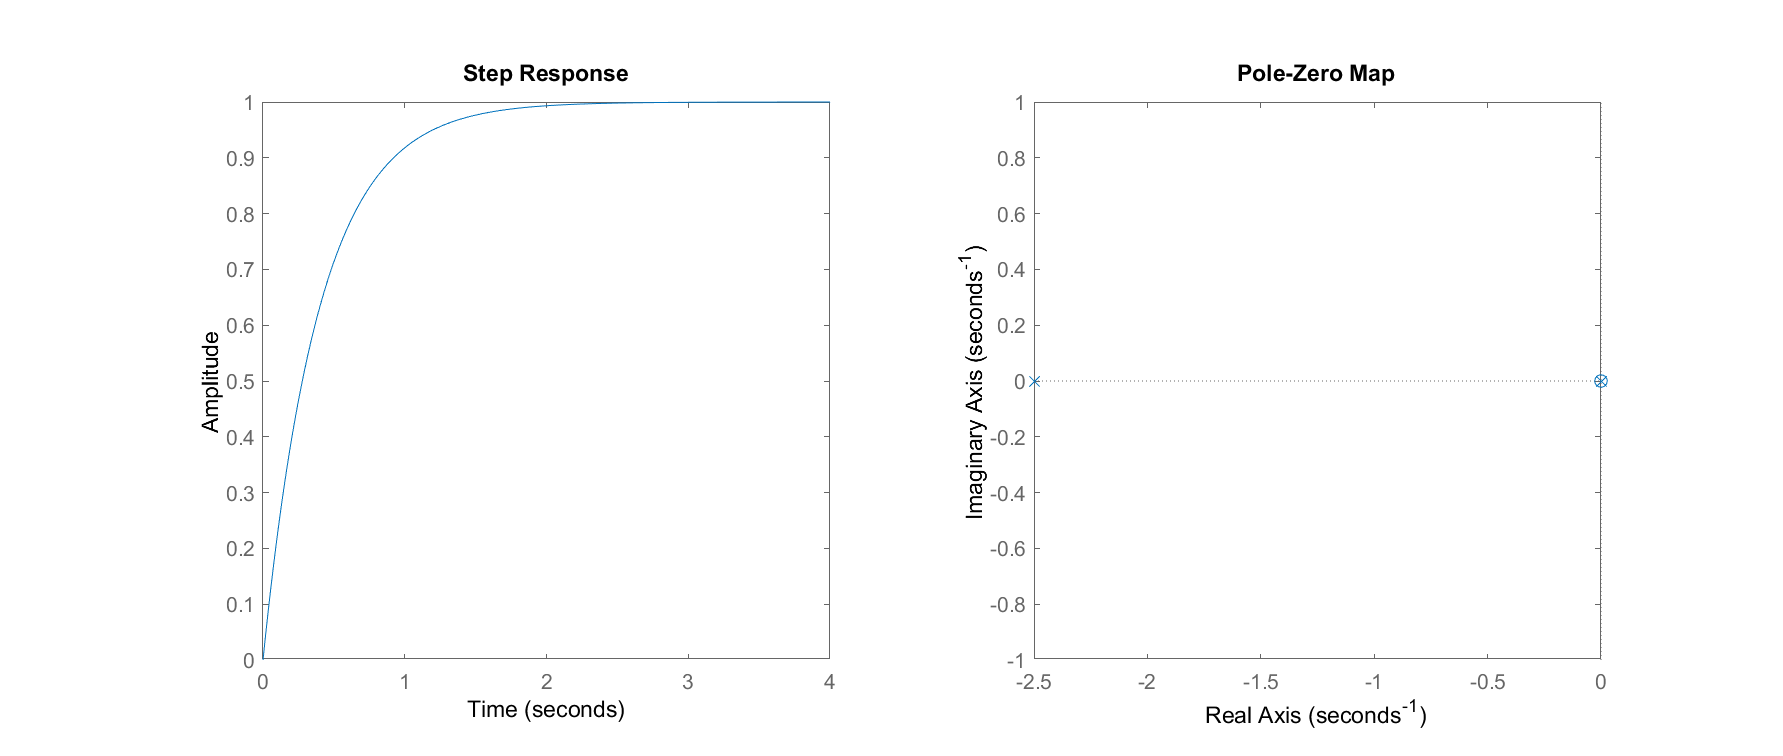
\includegraphics[width=1\textwidth]{no_controller.eps}
    \caption{Step-response and "poles and zero" plot for the system without controller}
    \label{fig:my_label}
\end{figure}

\end{frame}


%%%%%%%%%%%%%%%% new page %%%%%%%%%%%%%%%%%%%%%%


\begin{frame}{Stability Analysis - Continuous Time}
The \textbf{PD}-controller implementations goal is to improve on the closed-loop system. The transfer functions then become:

\begin{equation}
        \Rightarrow G_{ol}(s) = \frac{k_p + k_d s}{s*2r} 
    \end{equation}
    
    And the closed loop transfer function:
    
    \begin{equation}
         \Rightarrow G_{cl}(s) = \frac{s*2r(kd*s+kp)}{s*2r(s(k_d+2r)+k_p)} 
    \end{equation}
\end{frame}


%%%%%%%%%%%%%%%% new page %%%%%%%%%%%%%%%%%%%%%%




%%%%%%%%%%%%%%%% new page %%%%%%%%%%%%%%%%%%%%%%

\begin{frame}{Stability Analysis - Continuous Time}

    From the closed-loop it's easy to see that $-2r<k_d$ in order to not have a pole in the positive right plane. The \textbf{PD} controller is therefore set to
    
    \begin{equation}
         \begin{cases}
             k_p=&5  \\
              k_d=&-r
        \end{cases}  
    \end{equation}
    
\end{frame}


%%%%%%%%%%%%%%%% new page %%%%%%%%%%%%%%%%%%%%%%




\begin{frame}{Stability Analysis - Continuous Time}

\begin{figure}
    \centering
    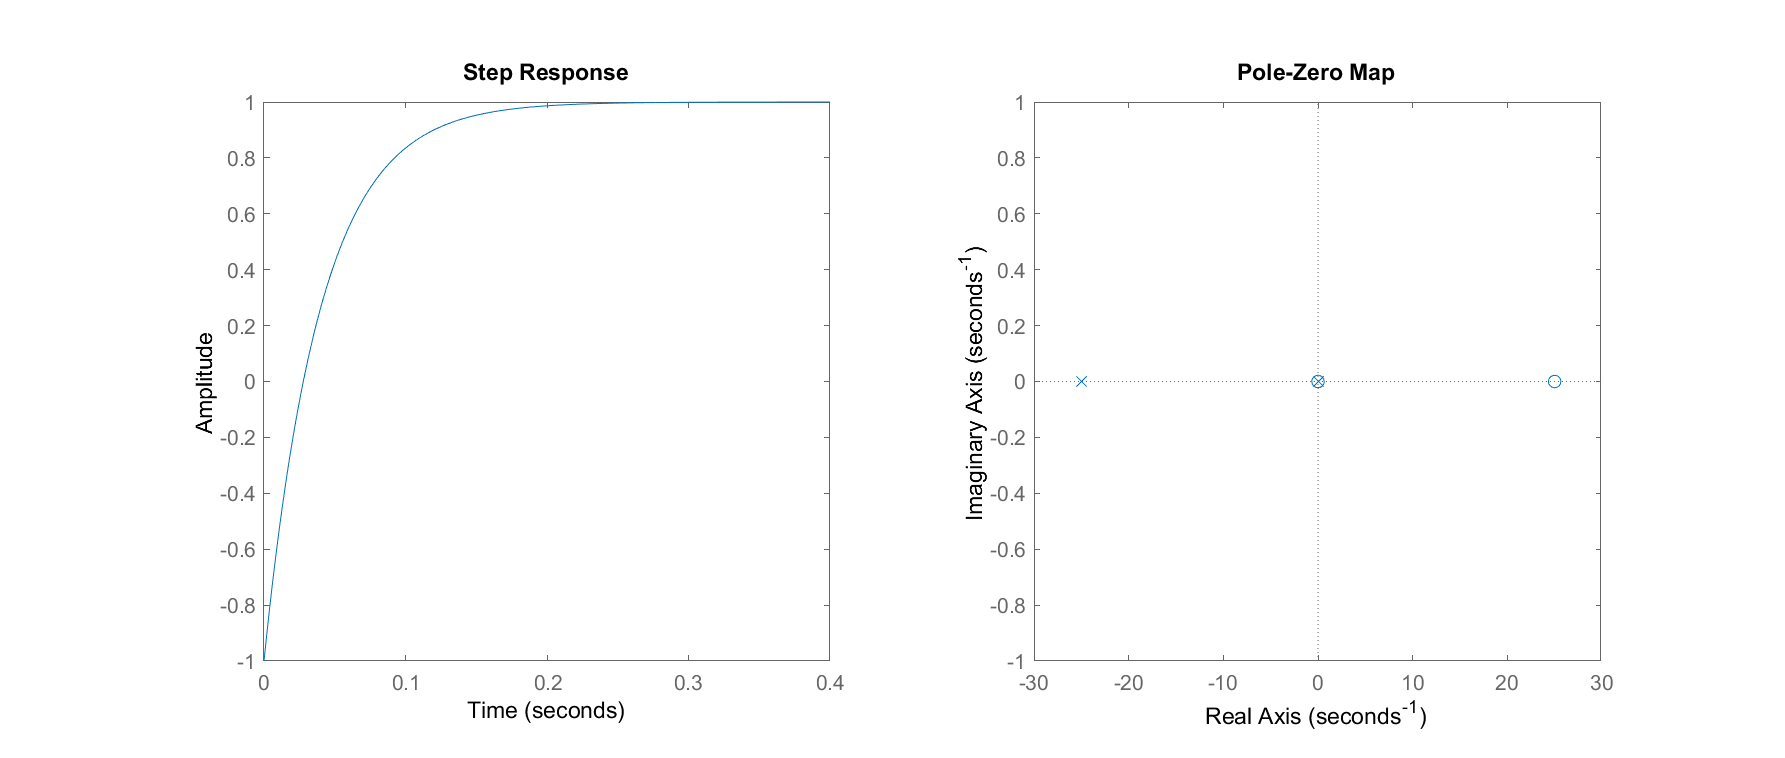
\includegraphics[width=1\textwidth]{PD_controller_stab.eps}
    \caption{Step-response and "poles and zero" plot for the system with \textbf{PD}-controller}
\end{figure}

\end{frame}

\begin{frame}{Stability Analysis - Continuous Time}
   \begin{columns}
   \begin{column}[]{0.5\textwidth}
  \textbf{Without controller}
  
  \begin{itemize}
      \item RiseTime: 0.8788 s
      \item SettlingTime: 1.5648 s
  \end{itemize}
   \end{column}
   \begin{column}[]{0.5\textwidth}
   \textbf{PD Controller}
   
    \begin{itemize}
      \item RiseTime: 0.0879 s
      \item SettlingTime: 0.1565 s
  \end{itemize}
   \end{column}
   \end{columns}
   The system is approx 10x faster with the controller.
   \end{frame}

\begin{frame}{Stability Analysis - Discrete Time}

    The \texttt{c2d} command in MATLAB was used to discretize the transfer function with a sampling rate of 20 Hz and a input delay of 1/30 seconds
    
    \begin{figure}
    \centering
    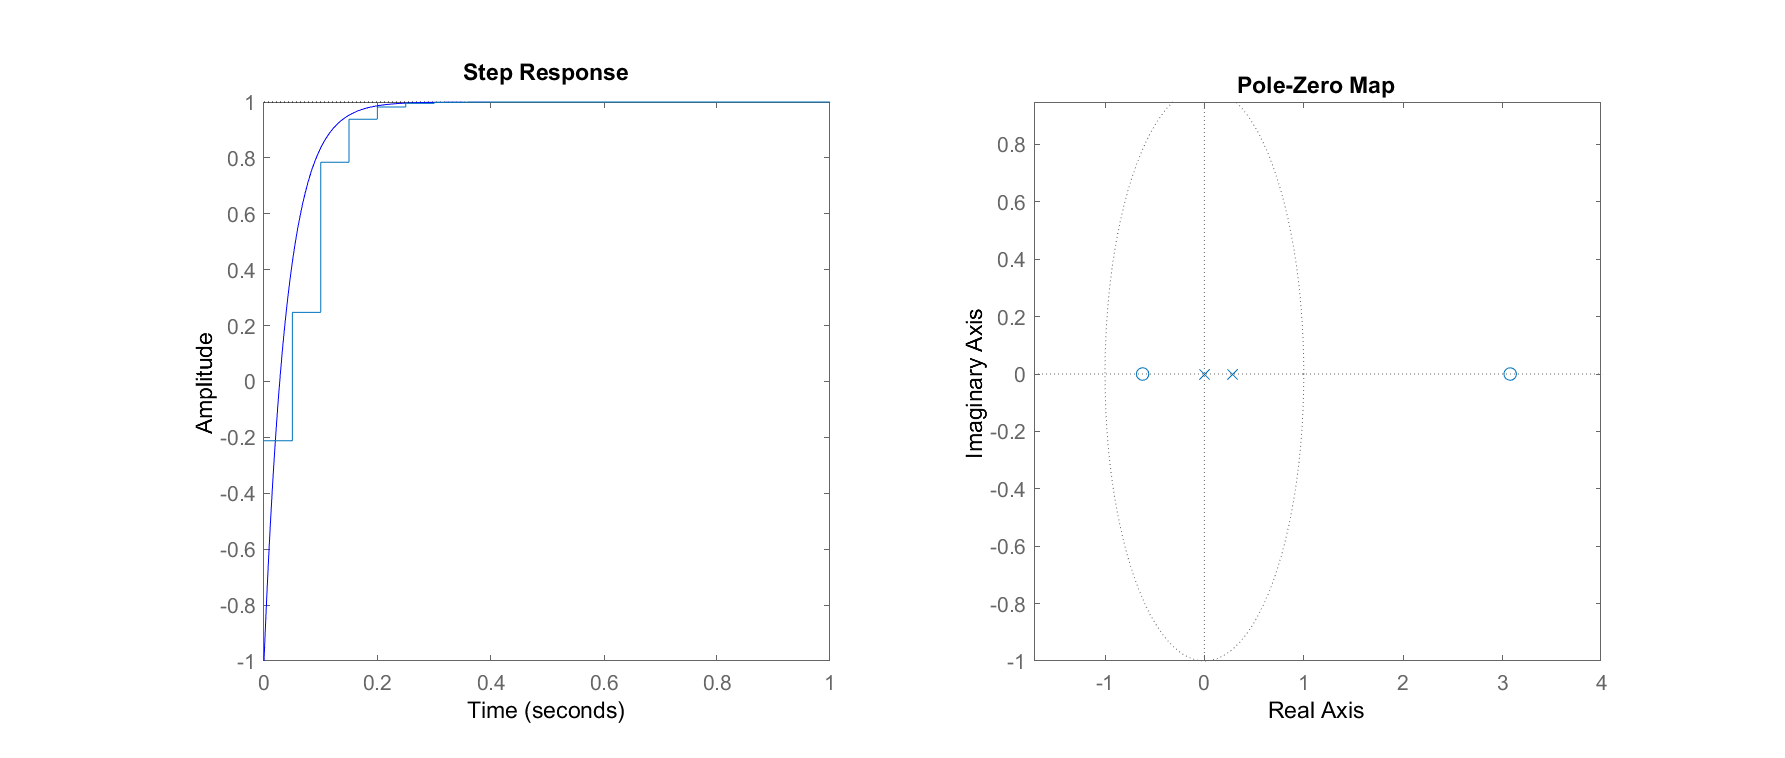
\includegraphics[width=1\textwidth]{PDd_controller_stab.eps}
    \caption{Step-response and "poles and zero" plot for the discrete system with a \textbf{PD}-controller}
\end{figure}

\end{frame}

\end{document}